\documentclass[11pt,a4paper]{article}

\usepackage[T1]{fontenc}
\usepackage[utf8]{inputenc}
\usepackage[english]{babel}
\usepackage[a4paper,top=2.35cm,bottom=2.45cm,left=2.55cm,right=2.55cm,headsep=12pt]{geometry}
\usepackage{amsmath,amssymb,mathtools}
\usepackage{enumitem}
\usepackage{eurosym}
\usepackage{graphicx}
\usepackage{xcolor}
\usepackage{microtype}
\usepackage{avant}
\usepackage{mathptmx}
\usepackage{titlesec}
\usepackage{fancyhdr}
\usepackage{mdframed}
\usepackage{tikz}
\usepackage{needspace}
\usepackage{hyperref}
\usetikzlibrary{arrows.meta,positioning}

\definecolor{PPEBurgundy}{RGB}{112,28,47}
\definecolor{PPENavarraRed}{RGB}{211,32,46}
\definecolor{PPEGold}{RGB}{185,143,57}
\definecolor{PPEAccentLight}{RGB}{248,235,238}
\definecolor{PPEInk}{RGB}{37,31,33}
\definecolor{PPEMuted}{RGB}{101,83,88}

\hypersetup{colorlinks=true,linkcolor=PPEBurgundy,urlcolor=PPEBurgundy}
\setlength{\parindent}{0pt}
\setlength{\parskip}{0.45em}
\setlist[itemize]{topsep=0.3em,itemsep=0.2em,leftmargin=1.5em}
\setlist[enumerate]{topsep=0.35em,itemsep=0.35em,leftmargin=1.9em}
\raggedbottom
\allowdisplaybreaks[2]

\titleformat{\section}{\sffamily\bfseries\large\color{PPEInk}}{\color{PPEBurgundy}\thesection}{0.8em}{}
\titlespacing*{\section}{0pt}{1.45em}{0.55em}

\newmdenv[
  skipabove=0.7em,skipbelow=0.9em,leftline=true,rightline=false,topline=false,bottomline=false,
  linewidth=3pt,linecolor=PPEBurgundy,backgroundcolor=PPEAccentLight,
  innerleftmargin=0.8em,innerrightmargin=0.8em,innertopmargin=0.55em,innerbottommargin=0.55em
]{solutionbox}
\newmdenv[
  skipabove=0.65em,skipbelow=0.75em,leftline=true,rightline=false,topline=false,bottomline=false,
  linewidth=2pt,linecolor=PPEGold,backgroundcolor=white,
  innerleftmargin=0.75em,innerrightmargin=0.75em,innertopmargin=0.45em,innerbottommargin=0.45em
]{tipbox}

\pagestyle{fancy}
\fancyhf{}
\fancyhead[LE,LO]{\sffamily\small Microeconomics \textbar{} Exercise Set II \textbar{} Worked solutions}
\fancyhead[RE,RO]{\sffamily\small\color{PPEBurgundy}\thepage}
\fancyfoot[C]{\sffamily\scriptsize\color{PPEMuted}Companion to Exercise Set II, Version B}
\renewcommand{\headrulewidth}{0.45pt}
\renewcommand{\headrule}{\hbox to\headwidth{\color{PPEGold}\leaders\hrule height \headrulewidth\hfill}}
\setlength{\headheight}{15pt}
\newcommand{\MRTS}{\operatorname{MRTS}}
\newcommand{\MPL}{\operatorname{MP}_{L}}
\newcommand{\MPK}{\operatorname{MP}_{K}}

\begin{document}

\begin{center}
  
\includegraphics[width=0.28\textwidth]{assets/branding/unav-logo-black.png}\par
  \vspace{0.55em}
  {\sffamily\color{PPENavarraRed}\large\textsc{Politics, Philosophy and Economics}\par}
  \vspace{0.3em}
  {\color{PPEGold}\rule{0.72\textwidth}{1.3pt}\par}
  \vspace{0.55em}
  {\sffamily\bfseries\color{PPEBurgundy}\LARGE Microeconomics: Exercise Set II\par}
  \vspace{0.16em}
  {\sffamily\large Worked solutions --- Version B --- Chapters 6--13\par}
\end{center}

\begin{solutionbox}
\textbf{How to use this key.} Attempt each question before consulting the solution.
The worked answers show the set-up, calculation, conclusion, and economic
interpretation. Equivalent algebra and clearly labelled diagrams are also valid.
\end{solutionbox}

\section{Individual and market demand}

\textbf{1.a Horizontal aggregation.} Consumer A buys only for \(p<9\), while
consumer B buys for \(p<12\). Since consumers face the same market price, add
their quantities:
\[
Q(p)=
\begin{cases}
30-3p, & 0\leq p<9,\\[0.35em]
12-p, & 9\leq p<12,\\[0.35em]
0, & p\geq12.
\end{cases}
\]
The individual choke prices are \(\boxed{9}\) and \(\boxed{12}\). At \(p=9\),
A leaves the market and B still demands 3 units, so \(p=9\) is the interior
kink. The market choke price is \(\boxed{12}\). With quantity on the
horizontal axis and price on the vertical axis, the curve passes through
\[
(Q,p)=(30,0),\qquad(3,9),\qquad(0,12).
\]

\begin{center}
\begin{tikzpicture}[x=0.18cm,y=0.34cm,>=Latex]
  \draw[->,thick] (0,0) -- (34,0) node[right] {quantity \(Q\)};
  \draw[->,thick] (0,0) -- (0,14) node[above] {price \(p\)};
  \draw[PPEBurgundy,very thick] (30,0) -- (3,9) -- (0,12);
  \filldraw[PPENavarraRed] (3,9) circle (2.2pt);
  \draw[densely dashed,PPEMuted] (3,0) -- (3,9) -- (0,9);
  \node[below] at (30,0) {\(30\)};
  \node[below] at (3,0) {\(3\)};
  \node[left] at (0,9) {\(9\)};
  \node[left] at (0,12) {\(12\)};
\end{tikzpicture}
\end{center}

\textbf{1.b Income and own-price changes.} Because
\[
\frac{\partial q_{\mathrm{bus}}}{\partial I}=-0.015<0,\qquad
\frac{\partial q_{\mathrm{coffee}}}{\partial I}=0.01>0,
\]
bus trips are \textbf{inferior} and coffee is \textbf{normal}. A change in the
price of a bus trip produces a movement along the demand curve. Changes in
income, the price of train travel, tastes, or population shift it.

\begin{solutionbox}
\textbf{Result.} The aggregate demand curve has a kink at \(p=9\), and its
final choke price is \(p=12\).
\end{solutionbox}

\section{Elasticity and revenue}

\textbf{2.a Point elasticity.} For \(q=120-3p\), \(dq/dp=-3\), hence
\[
\varepsilon_{q,p}=-3\frac{p}{120-3p}.
\]
\[
\begin{array}{c|c|c|c}
p&q&\varepsilon_{q,p}&TR=pq\\ \hline
10&90&-\frac13\ \text{(inelastic)}&900\\
20&60&-1\ \text{(unit elastic)}&1200\\
30&30&-3\ \text{(elastic)}&900
\end{array}
\]

\textbf{2.b Arc elasticity.} Between \(p=10\) and \(p=20\),
\[
\varepsilon_{\mathrm{arc}}
=\frac{(60-90)/[(60+90)/2]}{(20-10)/[(20+10)/2]}
=\frac{-30/75}{10/15}=\boxed{-0.6}.
\]
Revenue is largest at \(p=20\), where demand is unit elastic. Equivalently,
\(TR=120p-3p^2\), and its derivative \(120-6p\) is zero at \(p=20\).

\textbf{2.c Cross-price elasticity.} A 12\% increase in coffee's price raises
tea demand by 6\%, so
\[
\varepsilon_{\mathrm{tea,coffee}}=\frac{6\%}{12\%}=\boxed{+0.5}.
\]
Tea and coffee are substitutes.

\section{Production technology}

\textbf{3.a Marginal products and technical substitution.} For
\(q=4L^{1/2}K^{1/2}\),
\[
\MPL=2\sqrt{\frac{K}{L}},\qquad
\MPK=2\sqrt{\frac{L}{K}},\qquad
\MRTS_{L,K}=\frac{\MPL}{\MPK}=\frac{K}{L}.
\]
At \((L,K)=(4,9)\),
\[
q=\boxed{24},\qquad \MPL=\boxed{3},\qquad
\MPK=\boxed{\frac43},\qquad \MRTS_{L,K}=\boxed{\frac94}.
\]
Thus another unit of labour produces three more units of output locally if
capital is held fixed.

\textbf{3.b Returns to scale.} Since
\[
f(2L,2K)=4\sqrt{(2L)(2K)}=2f(L,K),
\]
the technology has \textbf{constant returns to scale}.

\textbf{3.c Isoquant.} For \(q=24\), \(4\sqrt{LK}=24\), so
\[
\boxed{K=\frac{36}{L}}.
\]
It is downward sloping and convex: the firm can replace some capital with
labour while holding output fixed, but the trade-off changes along the curve.

\section{Cost minimisation and economic cost}

\textbf{4.a Isocost.} With \(w=4\) and \(r=1\),
\[
C=4L+K.
\]
For \(C=60\), the line is \(K=60-4L\), with intercepts \((15,0)\) and
\((0,60)\) and slope \(-4\).

\textbf{4.b Conditional factor demand.} At an interior minimum,
\[
\MRTS_{L,K}=\frac{K}{L}=\frac{w}{r}=4
\quad\Longrightarrow\quad K=4L.
\]
Together with \(\sqrt{LK}=12\),
\[
\sqrt{4L^2}=2L=12
\quad\Longrightarrow\quad
\boxed{L^*=6,\qquad K^*=24}.
\]
Therefore,
\[
C^*=4(6)+24=\boxed{48}.
\]

\textbf{4.c Economic cost.} An office that the entrepreneur owns can be rented
out for \euro500 per month. The forgone rent is not an accounting expense if no
cash is paid, but it is an opportunity cost. Economic profit is consequently
\euro500 lower than accounting profit.

\section{Cost curves and the shutdown decision}

For \(TC(q)=80+5q+q^2\),
\[
FC=80,\qquad VC=5q+q^2,\qquad AVC=5+q,
\]
\[
ATC=\frac{80}{q}+5+q,\qquad MC=5+2q.
\]

\textbf{5.a Price \(p=21\).} Set price equal to marginal cost:
\[
21=5+2q\quad\Longrightarrow\quad\boxed{q^*=8}.
\]
Then \(TR=168\), \(TC=184\), and \(\pi=\boxed{-16}\). The firm should still
operate in the short run because it covers variable cost and contributes to
fixed cost.

\textbf{5.b Price \(p=4\).} The minimum average variable cost is 5 (approached
as \(q\) approaches zero). Since \(4<5\), the firm shuts down.

\begin{solutionbox}
\textbf{Short-run supply.}
\[
q_s(p)=
\begin{cases}
0, & p\leq5,\\[0.3em]
\dfrac{p-5}{2}, & p>5.
\end{cases}
\]
At \(p=5\), the usual supply convention records zero output.
\end{solutionbox}

\section{Competitive equilibrium and a tax}

\textbf{6.a Untaxed market.} Equating \(Q_D=100-2P\) and \(Q_S=2P-20\),
\[
100-2P=2P-20
\quad\Longrightarrow\quad\boxed{P^*=30,\qquad Q^*=40}.
\]
Demand's choke price is 50 and supply's intercept is 10. Therefore
\[
CS=\tfrac12(50-30)(40)=400,\qquad
PS=\tfrac12(30-10)(40)=400,
\]
so total surplus is \(\boxed{800}\).

\textbf{6.b Tax of \(t=8\).} Let \(p_B-p_S=8\). Then
\[
100-2(p_S+8)=2p_S-20
\quad\Longrightarrow\quad
\boxed{p_S=26,\quad p_B=34,\quad Q=32}.
\]
Tax revenue is \(8(32)=\boxed{256}\), while
\[
\boxed{DWL=\tfrac12(40-32)(8)=32}.
\]
Demand and supply have equal absolute slopes, so buyers pay \euro4 more and
sellers receive \euro4 less per unit.

\begin{center}
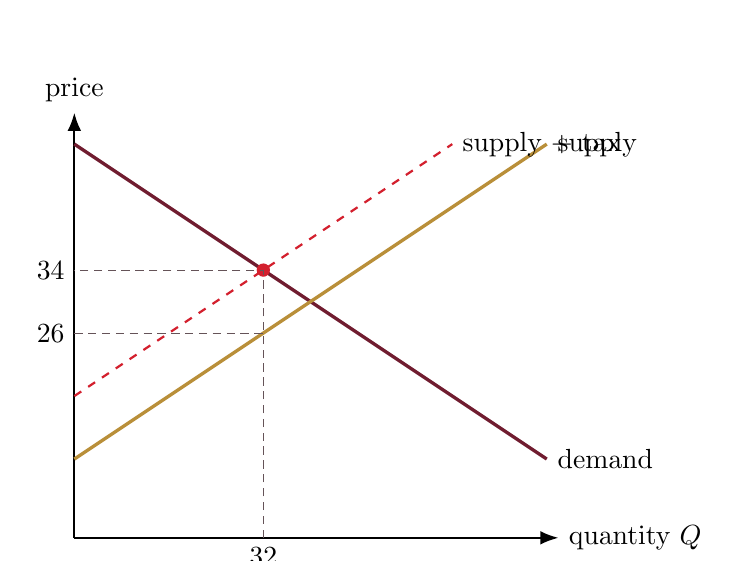
\begin{tikzpicture}[x=0.075cm,y=0.10cm,>=Latex]
  \draw[->,thick] (0,0) -- (82,0) node[right] {quantity \(Q\)};
  \draw[->,thick] (0,0) -- (0,54) node[above] {price};
  \draw[PPEBurgundy,very thick] (0,50) -- (80,10) node[right,black] {demand};
  \draw[PPEGold,very thick] (0,10) -- (80,50) node[right,black] {supply};
  \draw[PPENavarraRed,thick,dashed] (0,18) -- (64,50) node[right,black] {supply + tax};
  \filldraw[PPENavarraRed] (32,34) circle (2.2pt);
  \draw[densely dashed,PPEMuted] (32,0) -- (32,34) -- (0,34);
  \draw[densely dashed,PPEMuted] (0,26) -- (32,26);
  \node[below] at (32,0) {\(32\)};
  \node[left] at (0,26) {\(26\)};
  \node[left] at (0,34) {\(34\)};
\end{tikzpicture}
\end{center}

\section{Monopoly and price discrimination}

For \(p=90-Q\) and \(C(Q)=30+10Q\),
\[
TR=90Q-Q^2,\qquad MR=90-2Q,\qquad MC=10.
\]

\textbf{7.a Monopoly choice.} Set \(MR=MC\):
\[
90-2Q=10\quad\Longrightarrow\quad Q_M=40,\qquad P_M=50.
\]
Profit is
\[
\pi_M=50(40)-[30+10(40)]=\boxed{1570}.
\]

\textbf{7.b Competitive benchmark.} Competition sets \(p=MC=10\), giving
\(Q_C=80\). Monopoly deadweight loss is
\[
\boxed{DWL=\tfrac12(80-40)(50-10)=800}.
\]

\begin{center}
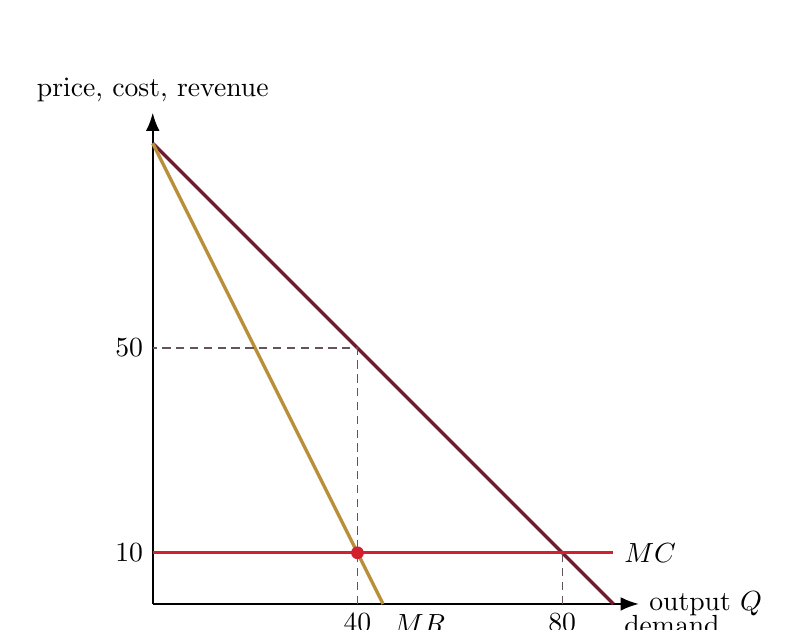
\begin{tikzpicture}[x=0.065cm,y=0.065cm,>=Latex]
  \draw[->,thick] (0,0) -- (95,0) node[right] {output \(Q\)};
  \draw[->,thick] (0,0) -- (0,96) node[above] {price, cost, revenue};
  \draw[PPEBurgundy,very thick] (0,90) -- (90,0) node[below right,black] {demand};
  \draw[PPEGold,very thick] (0,90) -- (45,0) node[below right,black] {\(MR\)};
  \draw[PPENavarraRed,very thick] (0,10) -- (90,10) node[right,black] {\(MC\)};
  \filldraw[PPENavarraRed] (40,10) circle (2.1pt);
  \draw[densely dashed,PPEMuted] (40,0) -- (40,50) -- (0,50);
  \draw[densely dashed,PPEMuted] (80,0) -- (80,10);
  \node[below] at (40,0) {\(40\)};
  \node[below] at (80,0) {\(80\)};
  \node[left] at (0,10) {\(10\)};
  \node[left] at (0,50) {\(50\)};
\end{tikzpicture}
\end{center}

\textbf{7.c Price discrimination.} The firm needs market power, a way to
identify or sort buyers with different willingness to pay, and an ability to
prevent resale. It can increase output and reduce deadweight loss, but the
distribution of surplus may still favour the firm.

\section{Cournot competition}

With \(p(Q)=80-Q\), \(Q=q_1+q_2\), and \(C_i(q_i)=20+20q_i\),
\[
\pi_i=(80-q_i-q_j)q_i-(20+20q_i)=(60-q_i-q_j)q_i-20.
\]

\textbf{8.a Reaction functions and equilibrium.} For firm 1,
\[
\frac{\partial\pi_1}{\partial q_1}=60-2q_1-q_2=0
\quad\Longrightarrow\quad q_1=30-\frac{q_2}{2}.
\]
By symmetry, \(q_2=30-q_1/2\). Solving gives
\[
\boxed{q_1^*=q_2^*=20,\qquad Q^*=40,\qquad p^*=40}.
\]
Each firm earns
\[
\pi_i=40(20)-[20+20(20)]=\boxed{380}.
\]

\begin{center}
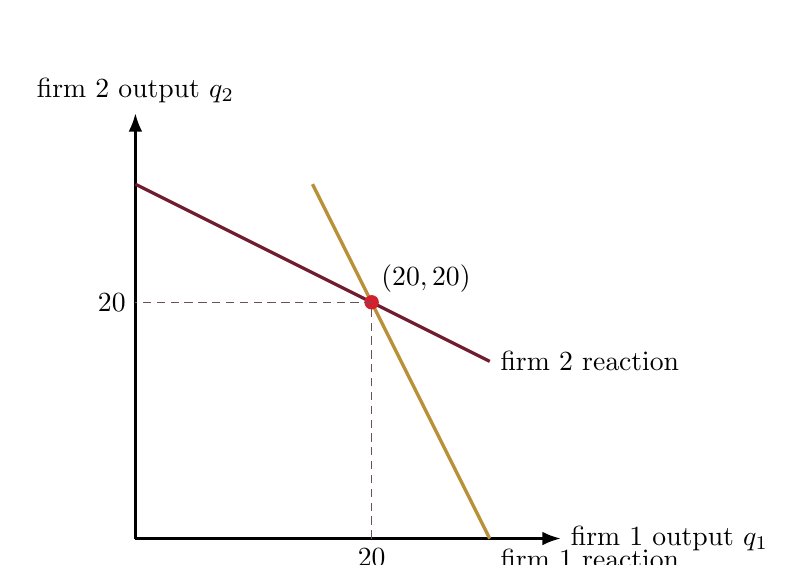
\begin{tikzpicture}[x=0.15cm,y=0.15cm,>=Latex]
  \draw[->,thick] (0,0) -- (36,0) node[right] {firm 1 output \(q_1\)};
  \draw[->,thick] (0,0) -- (0,36) node[above] {firm 2 output \(q_2\)};
  \draw[PPEBurgundy,very thick] (0,30) -- (30,15) node[right,black] {firm 2 reaction};
  \draw[PPEGold,very thick] (15,30) -- (30,0) node[below right,black] {firm 1 reaction};
  \filldraw[PPENavarraRed] (20,20) circle (2.4pt) node[above right,black] {\((20,20)\)};
  \draw[densely dashed,PPEMuted] (20,0) -- (20,20) -- (0,20);
  \node[below] at (20,0) {\(20\)};
  \node[left] at (0,20) {\(20\)};
\end{tikzpicture}
\end{center}

\textbf{8.b Comparison.} Monopoly gives \(Q_M=30\), \(P_M=50\); perfect
competition gives \(Q_C=60\), \(P_C=20\). Thus
\[
\boxed{Q_M=30<Q_{\mathrm{Cournot}}=40<Q_C=60},\qquad
\boxed{P_M=50>P_{\mathrm{Cournot}}=40>P_C=20}.
\]

\textbf{8.c Cartel temptation.} A cartel maximising joint profit would produce
the monopoly quantity 30, perhaps 15 each. But if the other firm produces 15,
a firm's best response is \(30-15/2=22.5\), not 15. Each firm is tempted to
expand secretly, which makes a cartel difficult to sustain.

\begin{solutionbox}
\textbf{Result.} Cournot equilibrium lies between monopoly and perfect
competition: firms produce more and charge less than a monopolist, but do not
reach the competitive outcome.
\end{solutionbox}

\end{document}

